\documentclass[11pt]{article}
\usepackage[margin=0.75in]{geometry}
\usepackage{amsmath}
\usepackage{physics}
\usepackage{listings}
\usepackage{caption}
\usepackage{graphicx}
\usepackage{algorithm}
\usepackage{algpseudocode}
\usepackage{setspace} \doublespacing
\usepackage{titling}
\graphicspath{{../Images/}}


\title{Emergence of Autocatalysis in Prebiotic Reaction Networks }
\author{Varun Varanasi \\{Advisor: Jun Korenaga}}
\begin{document}

\maketitle
\newpage

\tableofcontents

\newpage

\section{Abstract}

Origin of life research is heavily focused on bridging the knowledge gap between prebiotic synthesis and emergence of life. 
Theoretical models posit that this transition was facilitated through a series of chemical reactions characterized by their ability to self-replicate, self-sustain, self-assemble, and autocatalyze.
Given the scarcity of known abiotic autocatalytic reactions, research efforts are focused on studying the emergence of autocatalysis in prebiotic chemical systems. 
Previous research has found a phase transition in the probability of producing an autocatalytic set in a kauffman model as a function of expected number of catalyzations, but details about the dynamics and characterization of this phenomena still remain an open question.
The goal of this research is to elucidate this relationship and develop a more cohesive understanding of autocatalytsis in prebiotic chemistry.
In particular, this work focused on mapping network properties to the presence of autocatalytic sets, studying the stability of autocatalytic reaction networks, and characterizing the toplogy of autocatalytic sets in the space of all possible networks.
Stability and the topology of autocatalytic sets were evaluated by inducing random catalytic perturbations and evaluting the effect on autocatalytic subsets.
The results of these tests found that graph proximity to the food set and presence of two-cycles in reaction networks are highly indicative of autocatalytic sets.
Perturbation analysis reveals to us that large networks are relatively more stable and that pertrubations based on the food-set are more influential at small sizes.
Stability testing also strongly indicates that the network space is partitioned into clusters of autocatalytic sets.
Results produced in this paper suggest for further analysis of underlying clustering structure of autocatalytic sets in ambient network space.

\newpage

\section{Introduction}

\subsection{Motivation}

Abiogenesis or the origin of life can be roughly partitioned into three phases: 1) Prebiotic Earth, 2) Primordial Soup, and 3) Emergence of Life. 

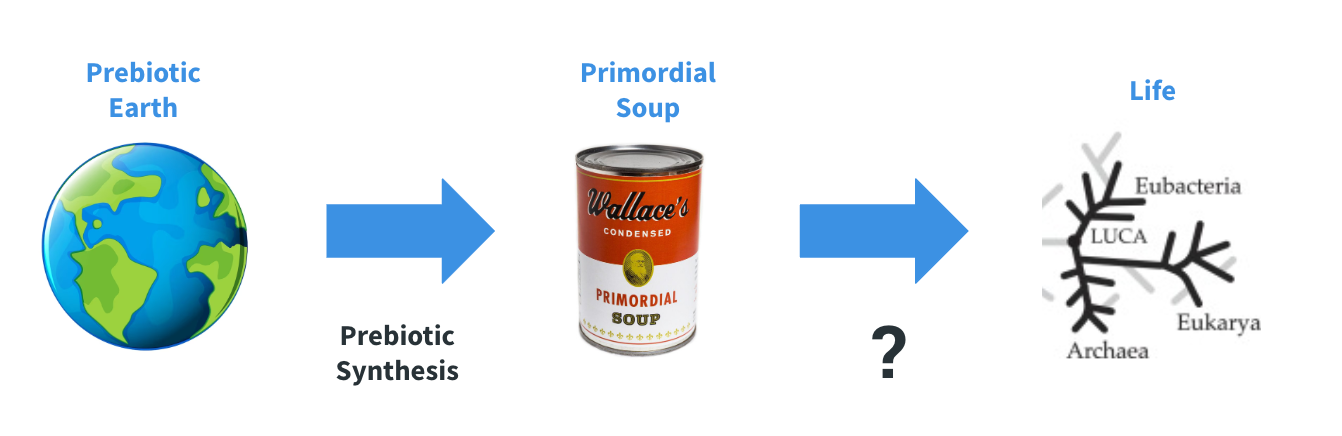
\includegraphics[width=\textwidth]{origin_of_life}

The first phase, labeled the Prebiotic Earth phase, occured approximately 4 billion years ago before life formed on Earth.
Still largely covered by liquid water, the Earth at this time was approximately 30\% dimmer than today with more x-ray and ultraviolet radiation.
The composition and chemistry of this time period still remains an open research question, but current theories characterize it as a weakly reducing atmosphere with an abundance of carbon dioxide and nitrogen, but very little oxygen.
All together, the conditions created an environment that was conducive to frequent ionization and an unstable atmosphere. \\

This environment was favorable for prebiotic synthesis, the process by which biotic molecules such as amino acids are created from abiotic precursors.
The mechanics and credibility of this process was a mystery until 1953 whe Stanley Miller and Harold Urey were able to replicate prebiotic synthesis in a University of Chicago laboratory.
Their experiment attempted to replicate the atmosphere of prebiotic earth by applying repeated sparks to a gas chamber of water, methane, ammonia, and hydrogen to replicate the action of lightning.
At the end of the experiment they were able to spontneously recover over 20 amino acids, the building blocks of proteins. 
This ground breaking experiment provided strong evidence supporting the prebiotic synthesis theory. \\

We believe that as biotic compounds accumulated via prebiotic synthesis, Earth's environment eventually entered a stage known as a primordial soup which was chracterized by the essential building blocks of life floating around the largely water covered Earth.
Life emerged from this soup; however, the process of this emergence still remains an open question.
Prevailing scinetific theories suggest that life initially began with the support of proton gradients provided by hydrothermal vents and eventually became LUCA or the Last Universal Common Ancestor from which all other organisms we know descended.  
Darwinian evolution provides us a strong understanding of this evolutionary process, but how LUCA and its precurosrs emerged from the primordial soup still remains a mystery.

My work focuses on answering this question. Theoretical models posit that these pseudo-supported life forms required a series of coupled self-sustaining, self-replicating, and autocatalyzing chemical reactions.
With the supoort of hydrothermal processes these reactions were eventually able to "evolve" into acutal life. 



\subsection{Background}

\subsubsection{Autocatalysis}
This work is focused on studying the process of autocatalysis. In particular, we want to understand its prevalence, the emergence, and dynamics so that we can uncover how, if at all, life originated from spontaneous chemical reactions in the primordial soup.

\begin{figure}[H]
    \centering
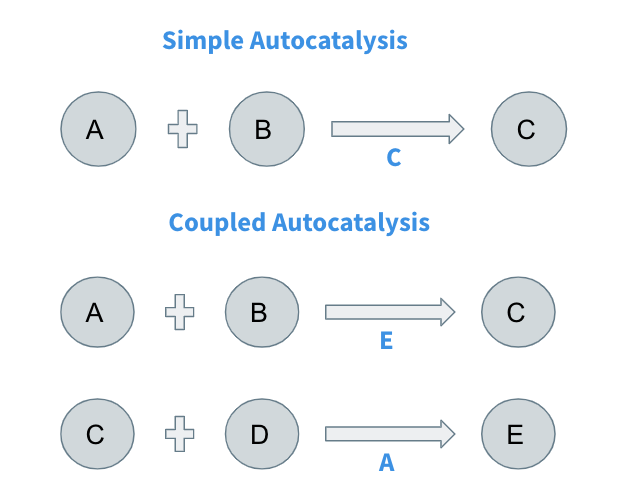
\includegraphics[width=8cm]{autocatalysis}
\caption{Autocatalysis}

\end{figure}

Autocatalysis, in its simplest definition, is a chemical reaction that is capable of catalyzing itself. 
In more general sitautions, autocatalysis can refer to a series of coupled reactions where each reaction is catalyzed by a product of another reaction in the reaction set. 
Autocatalytic reactions or autocatalytic sets function as positive feedback loops that are able to self-sustain and increase production as more products are produced. 
In the context of the origin of life, they are important in sustaining unfavorable chemical reactions and producing an abundance of molecular products prerequisite for life.

\subsubsection*{Reaction Networks}

Research is yet to discover an abiotic reaction capable of autocatalysis, so prebiotic autocatalysis research tends to focus on series of coupled chemical reactions. 
These systems are typically studied through reaction networks such as the one below. 

\begin{figure}[H]
    \centering
    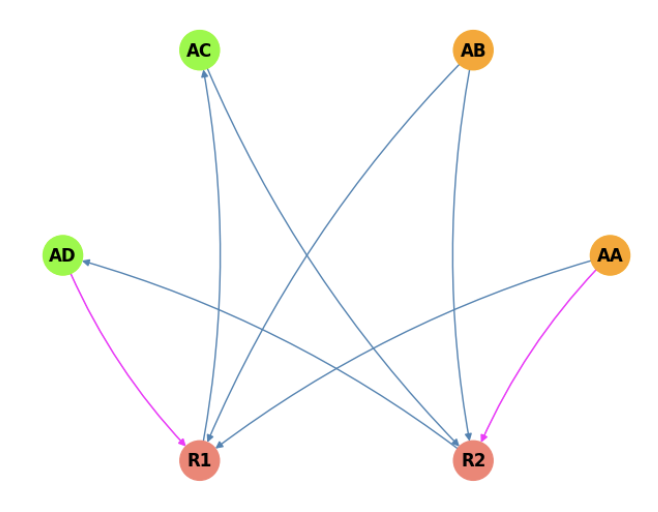
\includegraphics[width=8cm]{reaction_network}
    \caption{Reaction Network}
\end{figure}

We interpret the reaction network as follows. The yellow nodes represent the food set. These are the molecules that are ambient in the environment i.e. they do not need to be produced. 
The green nodes represent other molecules in a system. Finally, the red nodes represent reactions. Edges originating at a molecule vertex and ending at a reaction node represent the reactants of a given reaction.
Similarly, edges originating at a reaction node and ending at a molecule node represent a product. 
Putting it together, we see that R1 represents the reaction of $AA + AB \rightarrow AC$. 
The final details to note are the pink edges which represent catalyzation reactions. In the example above, we see that AD catalyzes R1 while AA catalyzes R2.
%With this understanding in mind, we can begin to discuss the Kauffman model, our model for prebiotic chemistry. 


\subsubsection{Kauffman Model}

The Kauffman model was developed by Stuart Kauffman in 1988 as a simplified representation of pre-biotic chemistry. 
Rather than focusing on actual chemical reactions, the essence of the model is to abstract chemical reactions into 4 sets of molecules and molecular relations.

\begin{itemize}
    \item X: The set of all possible molecules
    \item F: The set of food molecules
    \item R: The set of all possible reactions allowed
    \item C: The set of catalyzing relations
\end{itemize}

X, the set of all possible molecules, is typically defined by two paramters: t and n. t represents the size of the alphabet used in the model while n represents the maximum size of a molecule in our set. 
Therefore, X is the set of all possible configurations up to length n where each index takes t possible values.
Typically, t takes on the value of 2 which represents either a 0 or 1 in each index. Depending on the size of the model, n can take on a range of values. Therefore, each model has a total of $2^{n +1} -2$ molecules and as we increase n, the size of our model grows exponentially.
Next, F represents the food set. As explained above, the food set is a representation of ambient molecules in the environment. These are molecules that exist in a theoretical reservoir and can be used without replacement.
R is the set of possible reactions allowed. In the Kauffman model the allowed reactions are concatenation reactions and splitting reactions. In other words, if the joining of two molecules end to end produces another molecule in X, then that is a valid reaction.
Similarly, if we can split a molecule in X into two other molecules also in X we can define a splitting reaction.
The final component of the Kauffman model is C, the set of catalyzing reactions. Each reaction in R can be catalyzed by any molecule in X. Therefore, the size of C is given by $X \cross R$. 
Since X, F, and R are each static parameters defined by the model type, in our experiments we tend to vary C and study the resulting behavior.

\subsubsection{Autocatalytic and RAF Sets}

The kauffman model provides a framework for chemical reactions, but doesn’t provide any insight into autocatalytic sets. 
As we talked about earlier, autocatalytic sets are self-catalyzing reactions. 
Depending on how the catalyzation relations align, a given Kauffman network can potentially contain autocatalytic sets within it. 
To make our model more robust, we can further require that the reaction set is self-sustaining. In other words, in a given environment the autocatalytic set would be able to survive. 
One way of ensuring this is to make sure every molecule in the set is either from the food set (the set of ambient molecules) or produced by the food set through a reaction catalyzed by a molecule present in the set.
We call such a set RAF which stands for reflexively autocatalytic and food-generated set. 

\subsection{Previous Work}

Now, with our understanding of autocatalysis, reaction networks, the Kauffman model, and RAF sets we can quickly cover key results in the field.
Namely, we will discuss the discovery of a phase transition in the probability of finding an RAF set in a given Kauffman model.
Published in 2004, "Detecting Autocatalytic, self-sustaining sets in Chemical reaction systems" by Hordjik and Steele details a novel algorithm to detect RAF sets in chemical reaction systems.

In their work they explore the probability of RAF occurence as a function of a probability parameter p. For a pre-defined p, each trial randomly creates a Kauffman network where each possible catalyzing reaction is included in C with probability p.
Based on this parameter p, they define a secondary value $f = |R| \cdot p$ which is a measure of the expected number of catalyzations per molecule.
For varying f values, Hordjik and Steele tested the probability of finding an RAF set for multiple values of n. 

\begin{figure}[H]
    \centering
    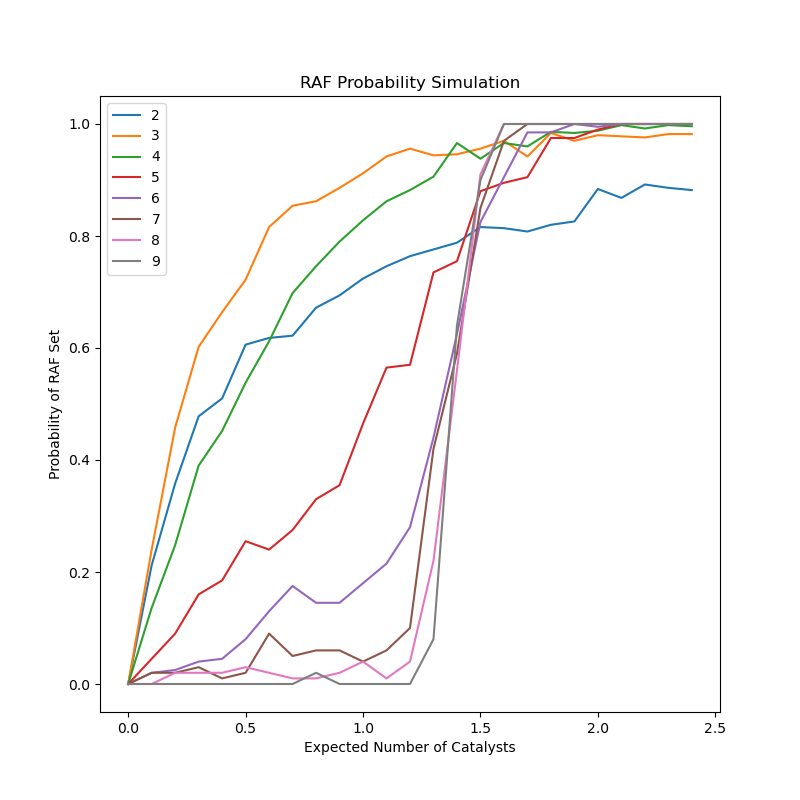
\includegraphics[width=12cm]{PhaseTransition.png}
    \caption{RAF Phase Transition}
\end{figure}

In particular, at $f =1.25$ the probability of detecting an RAF set jumps from near 0 to apprximately 100\%. 
Notice that as n increases the steepness of this jump increases. 
This apparent phase transition in the probability of an RAF set occuring is of great interest. 
The major focus of this thesis work is to characterize the networks around this phase transition and understanding the underlying structure of RAF sets.

\section{Classification}


\subsection{Methodology}

The first methodology used to study this apparent phase transition was to consider the presence of RAF networks as a purely statistical problem. 
For each network, we have set graph properties and a binary classification on whether the network contains an RAF set. 
Therefore, for a sufficiently large dataset, we can run a classification algorithm using a feature set of graph properties. 
In particular, we analyzed the following network properties across each of our simulations:

\begin{itemize}
        \item Number of nodes
        \item Number of Non-Food catalyzations
        \item Number of Food catalyzations
        \item $\Delta$ Network Diameter
        \item Number of Two cycles
        \item  $\Delta$ Betweeneess Centrality
        \item Number of Expected catalyzations
        \item Food Set to Node Ratio
\end{itemize}

Note that the $\Delta$ qualities refer to differences in the graph properties before and after adding catalyzation edges to the constructed network.


In total a dataset of 11,100 networks from size n = 2 to n = 7 of which approximately 64\% were RAF (7095) was created and analyzed.
This data was then used to train a logistic regression model to uncover the relative importance of each factor in predicting an RAF set.

\subsection{Results and Analysis}

Our logistic regression was able to produce a score of 80\% accuracy on a test set containin 25\% of the total dataset. 
The resulting coefficients can be found in the chart below:

\begin{figure}[H]
    \centering
    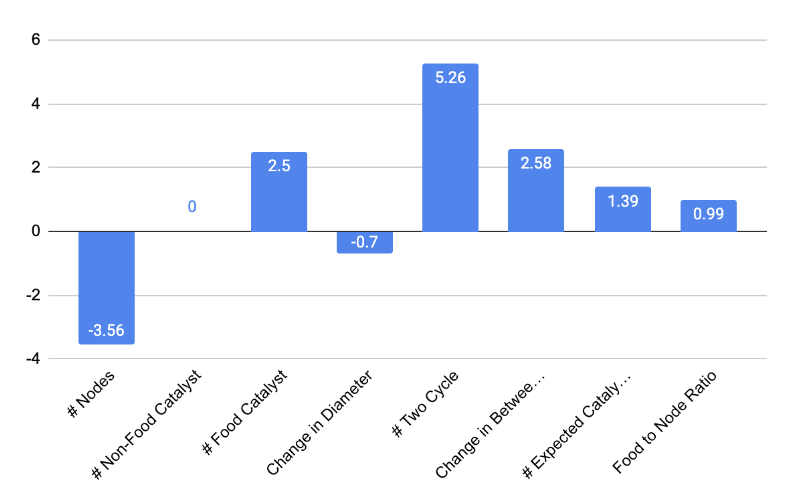
\includegraphics[width=15cm]{classification}
    \caption{Classification Results}
\end{figure}

Since we normalize the features before conducting the logistic regression, we cannot meaningfully apply the log-odds interpretation of logistic regression coefficients, but the relative differences between the values provides us insight into each features importance in predicting an RAF set.
From the chart it is clear that our three most prominent features are the number of two cycles, change in betweenness centrality, and number of food catalysts. 
Additionally, we see that the number of nodes is inversely related to the presence of an RAF set.  
Furthermore, we see that the number of two cycles is about twice as influential as either food catalysts or change in betweenness centrality.  

From our classification results it is apparent that proximity to the food set is highly predictive of finding RAF sets in the data. 
We also see that catalysts relations involving food set molecules are relatively more important than their counterparts.
Finally, we notice that two cycles or self-autocatalytic reactions are incredibly important in producing an RAF set/subset.

\section{Stability Across Probability Regimes}

\subsection{Methodology}

From Hordjik and Steele's work we know that RAF probability can be modeled as a function of probability of catalyzation, but what makes different networks successful in producing an RAF for the same probability? 
We propose answering this question by introducing the notion of RAF stability. In other words, how does a network respond to a perturbation of either adding or removing an edge?
In the case that we do not have an RAF set in our network, our perturbation adds an arbitrary catalyzing edge to the set. 
On the other hand, if we do have an RAF set in our network, our perturbation acts to remove a random catalyzing edge from the set. 
After doing so, we can look at the percentage of networks that remain in their existing state and quantify the "stability" of the RAF set. 

Note that from our work with classification we see that proximity and catalysts from the food set are incredibly important in determining the presence of an RAF set. 
With this in mind, we act to test a second hypothesis using food-set perturbations.
In other words, each perturbation acts to either add/remove food-set catalysts where applicable. 

We ran stability testing across 3 different probability regimes defined by their expected probabilitity of contianing an RAF set.
In particular, we tested expected RAF observation probabilities of approximately 30\%, 50\%, and 75\%. A summary of the number of trials run for each value of n can be found below.

\begin{table}[h!]
    \centering
     \begin{tabular}{||c| c||} 
     \hline
     Max Molecule Size (n) & Number of Trials \\ [0.5ex] 
     \hline\hline
     2 & 5000 \\ 
     3 & 2500 \\
     4 & 1000 \\
     5 & 1000 \\
     6 & 500 \\
     7 & 300 \\ [1ex] 
     \hline
    \end{tabular}
\end{table}

\subsection{Results and Analysis} 

\begin{center}
\begin{frame}
    \centering
      \begin{tabular}{c}
      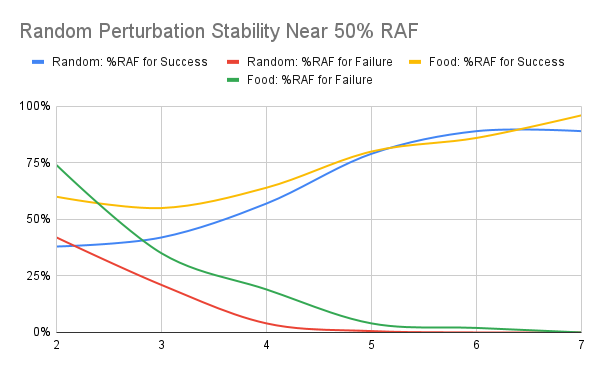
\includegraphics[width=9cm]{perturbation.png} \\
      50\% Probability Regime
    \end{tabular}

    \centering
    \vspace{0.01em}
      \begin{tabular}{cc}
      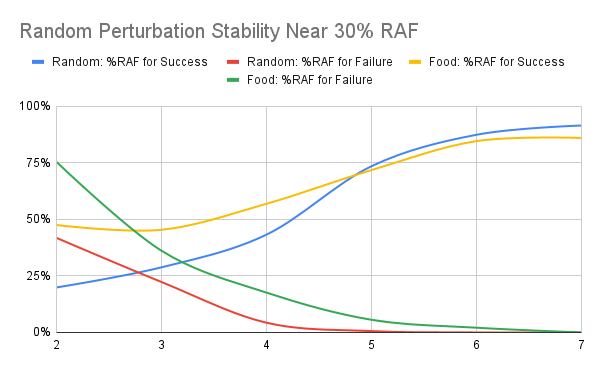
\includegraphics[width=9cm]{PerturbationLow.png}
       &
       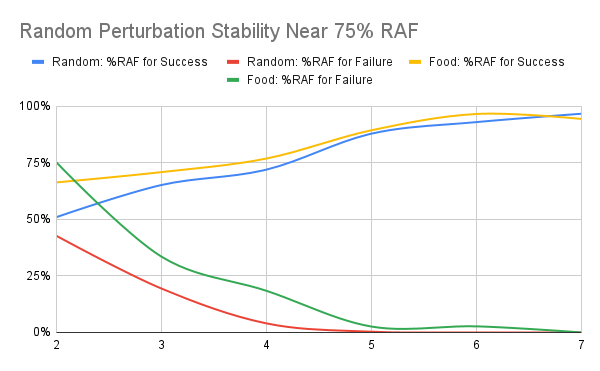
\includegraphics[width=9cm]{PerturbationHigh.png} \\
       30\% Probability Regime  & 75\% Probability Regime \\
       \end{tabular}
\end{frame}
\end{center}

Across all three regimes, as n increases, the influence of a single perturbation decreases. This large-autocatalytic network stability is rather intuitive since a single perturbation is a relatively smaller change as we increse network size.
This same observation holds for both RAF and Non-RAF sets implying that when a network is in a given state, it is resiliant to changing. 
This result can be further interpreted as evidence of clustering in the space of total networks as a single perturbation likely does not move a network out of the RAF/Non-RAF state.
If the RAF and Non-RAF sets were uniformly distributed we would expect perturbations to be more likely to inspire change. 
By looking at the different probability regimes we argue that this segmentation of network space increases as the expected probability of observing an RAF set increases. 
This statement is evidenced by the fact that there appears to be a slight increase in probability of not changing the state given a perturbation as we increase the expected observation probability.
Finally, we can also see that the food set perturbation is more influential than a random perturbation which corroborates our findings from the classification analysis. 
Furthermore, we can see that the influence of the food set perturbation is more pronounced at low n and levels off to match the random perturbation as n increases. 
It also appears that the random perturbation for success cases approaches an asymptotic bound, but more testing is needed to confirm whether this observation is a statistical artifact or representative of a deeper underlying phenomena.


\section{Absolute Stability}


\subsection{Methodology}

The natural next question following our results in the single perturbation stability testing is to ask how many random perturbations does it take to change the state of the system? 
With that in mind, we conducted a similar analysis to the previous section, but instead of limiting the perturbation to a single change, in the case of RAF sets, we repeatedly remove catalysts until the network is no longer autocatalytic. 
On the flip side, for Non-RAF sets, we repeatedly add random catalysts until an autocatalytic set emerges. 
Based on the results from the previous analysis in this phase we elect to drop our specific consideration of food-set catalysts.
We focused on the 50\% expected probability of RAF observation regime with the following trials:

\begin{table}[h!]
    \centering
     \begin{tabular}{||c| c| c||} 
     \hline
     Max Molecule Size (n) & Number of RAF Trials & Number of Non-RAF Trials \\ [0.5ex] 
     \hline\hline
     2 & 2451 & 2549 \\ 
     3 & 2514 & 2488 \\
     4 & 1075 & 926 \\
     5 & 1089 & 913 \\
     6 & 939 & 1065 \\
     7 & 596 & 410 \\ 
     8 & 615 & 89 \\ 
     9 & 18 & 4 \\ 
     \hline
    \end{tabular}
\end{table}



\subsection{Results and Analysis}

Our results were summarized via scaled histograms of the number of perturbations required to change the state of the system.
The x-axis in each graph is scaled by the number of total reactions in the network. 
This scaling effectively translates the number of perturbations to a multiple of network size so that the x-axis can be comapred across graphs. 
This analysis was conducted for both RAF and Non-Raf sets. 


\begin{figure}[H]
    \centering
    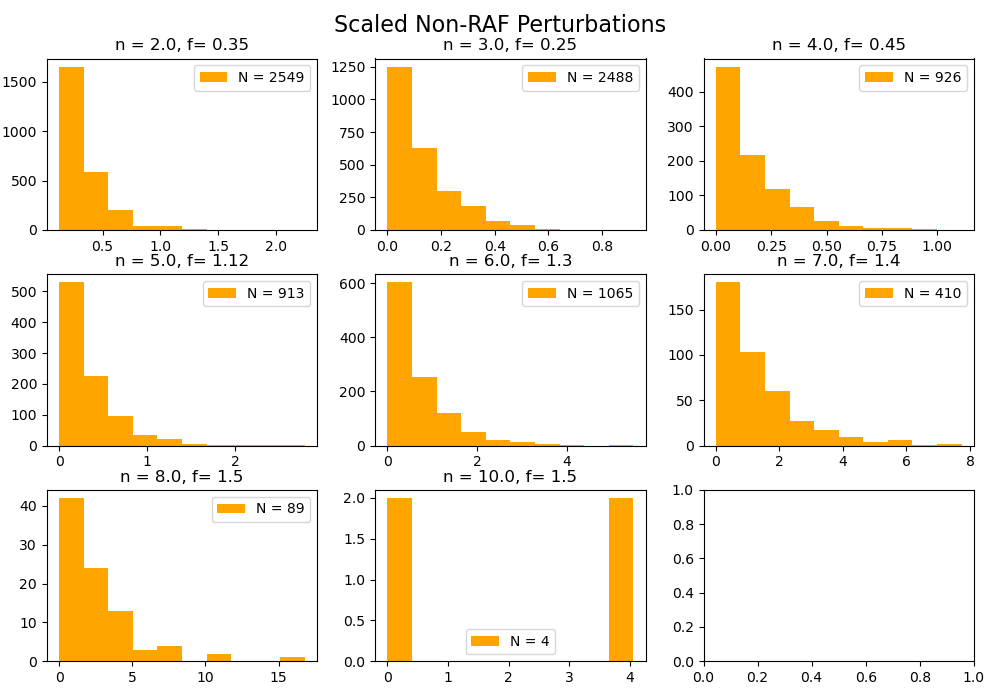
\includegraphics[width=15cm]{Scaled-Non-RAF_Perturbations_Hist.png}
    \caption{Non-RAF Absolute Stability Histograms}
\end{figure}
\begin{figure}[H]
    \centering
    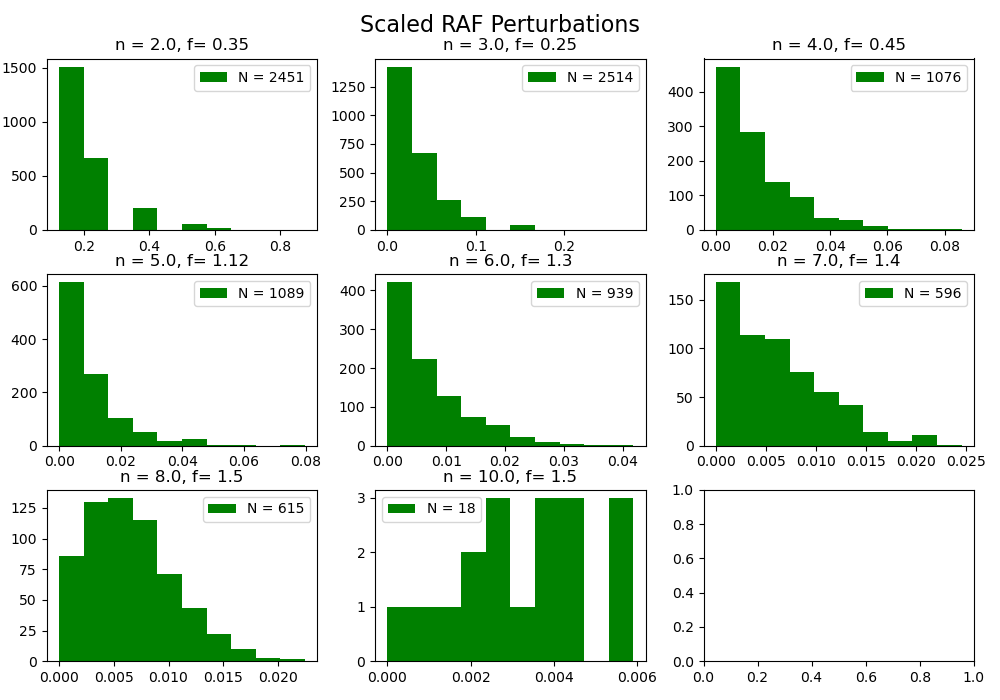
\includegraphics[width=15cm]{Scaled-RAF_Perturbations_Hist.png}
    \caption{RAF Absolute Stability Histograms}
\end{figure}

The structure of the histogram appears to be exponentially decreasing in number of scaled perturbations.
To extend the perturbation trend beyond the calculated data, we fit the distribution of perturbations to an exponential distribution via a mximum likelihood estimator.
If you recall, the exponential distribution is given by 

$$
f(x) = \lambda e^{\lambda x} \qquad x \geq 0 \qquad  0 \text{ otherwise}
$$

The corresponding log-likelihood function is given by 
$$\ell = n \ln(\lambda) - \lambda \sum_i x_i$$

This value is then maximized when $\hat{\lambda} = \frac{n}{\sum_i x_i}$.
Using this analysis we calculated the estimated exponential rate parameter for each value of n and f.
Our results are summarized via contour plots. As a note for interpretation, large values for the rate parameter correspond to sharp distributions while small values correspond to more evenly spaced out distributions.

\begin{figure}[H]
    \centering
    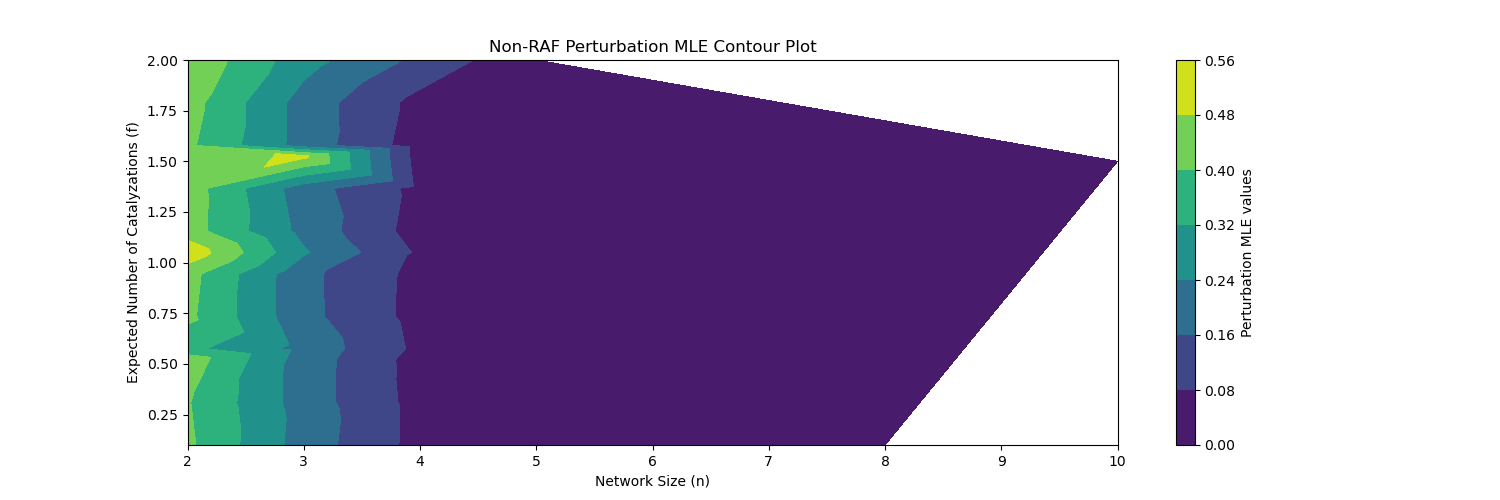
\includegraphics[width=15cm]{MLE_Contour_Non-RAF_Perturbation.png}
    \caption{Non-RAF MLE Coutour Plot}
\end{figure}
\begin{figure}[H]
    \centering
    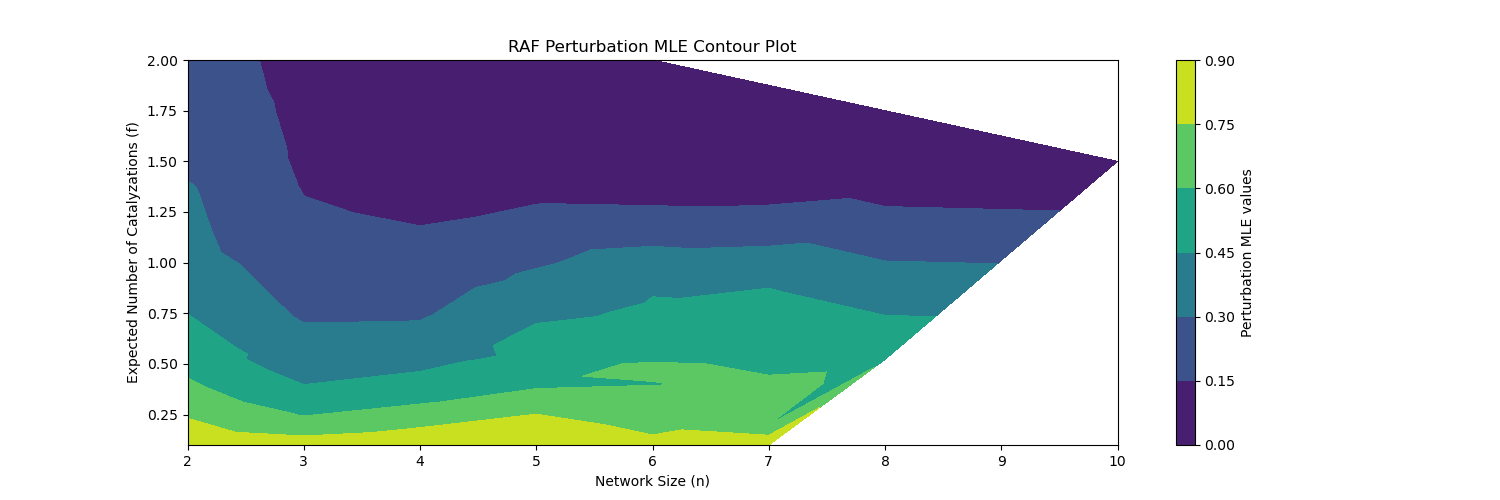
\includegraphics[width=15cm]{MLE_Contour_RAF_Perturbation.png}
    \caption{RAF MLE Contour Pot}
\end{figure}

The key observation from these results is that scaled Non-RAF perturbations occur on a different order of magnitude than their RAF counterparts. 
Specifically, Non-RAF perturbations occur on the order of 1 or 2 scaled counts while RAF counts occur around 0.01 scaled counts.
In terms of the topology of the space of RAF and Non-RAF sets, we can infer that the Non-RAF set is much more expansive than the RAF spaces. 
Alternatively, we say that the distance between the average Non-RAF set to an RAF set is much larger than the distance from an average RAF set to a Non-RAF set.
Furthermore, the ratio of these distances appear to be constant with increases in network size.
Finally, as expected, the variance in the number of perturbations required to change state increases with network size.
Together, these conclusions lead us to believe that the toplogical space of these networks is highly structured. 


\section{Conclusion}

This work has found a strong correlation between graph properties, particularly proximity measurements between food set and the rest of the graph, and the presence of RAF sets. 
These results point us in the direction that the food-set may play a larger role in the emregence of RAF sets than previously considered. 
Similarly, the discovery of the importance of two-cycles in RAF emergence may be indicitive of a model flaw, as two-cycles represent physically improbable situations.
If we are trying to model complex coupled autocatalytic reactions that exist in nature, relying on self-catalyzing reactions in the form of two-cycles may obscure our study of actual prebiotic autocatalytic emergence. 
Our perturbation analysis further reveal to us that large kauffman networks are stable to singular modifications. 
In other words, if an autocatalytic set is able to be produced containing many molecules, it is difficult to disturb this set. 
In our understanding of prebiotic chemistry, this could indicate to us that the probabilistic bottleneck in autocatalytic reaction networks is not in the larger scale, but rather in smaller networks as the develop.
Our perturbation analysis also indicates that the toplogical space of these networks is structured with RAF clusters distributed across the space of all possible networks.
It appears that the relative size of these RAF clusters to the network space remains constant as we increase network complexity.



\section{Further Work}

My thesis work provides strong evidence towards the existence of RAF clusters in the space of Kauffman networks. 
My future directions of research are to evaluate the topological structure through clustering analysis and evaluation of RAF cores, subsets of stable RAF networks built RAF networks. 
I am also interested to see how our results about the importance of food-set reactions propogate to clustering behavior.
In particular, I am interested in studying how RAF sets cluster around food-set catalysts. 
Finally, there appears to be a fundamental connection to percolation theory that would be fruitful to explore.
Doing so will ground this work with a storng theoretical foundation and allow rigorous analysis at scale.



\section{Acknowledgment}

I would like to thank Prof. Jun Korenaga for giving me the opportunity to work on this project. He has been an invaluable mentor and endlessly supportive throughout the process. 
I would also like to thank the Yale Physics department for its support and resources over the last four years.

\end{document}